% ---------------------------------------------------------
% Project: PhD KAPPA
% File: appendix.tex
% Author: Andrea Discacciati
%
% Purpose: Appendix
% ---------------------------------------------------------

\chapter{Supplementary figures}

\begin{sidewaysfigure}
\centering
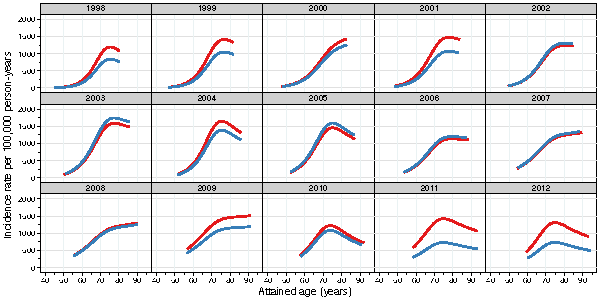
\includegraphics[width=\linewidth]{figures/appendix_ir_cosm.pdf}
\caption[Incidence rate of prostate cancer in the COSM by calendar year, attained age, and enrollment county]{Incidence rate of prostate cancer in the COSM, conditional on calendar year, attained age, and enrollment county (Västmanland/Örebro). The red line is the model-based predicted incidence rate for Västmanland county. The blue line is the model-based predicted incidence rate for Örebro county. The IRs between the 2 counties are forced to be proportional within calendar year. The $p_{\textrm{heterogeneity}}$ of the $\mathrm{IRR}_{\textrm{Västmanland vs. Örebro}}$ by calendar year was less than 0.001.}
\label{fig:appendix_ir_cosm}
\end{sidewaysfigure}

\begin{figure}[p]
\centering
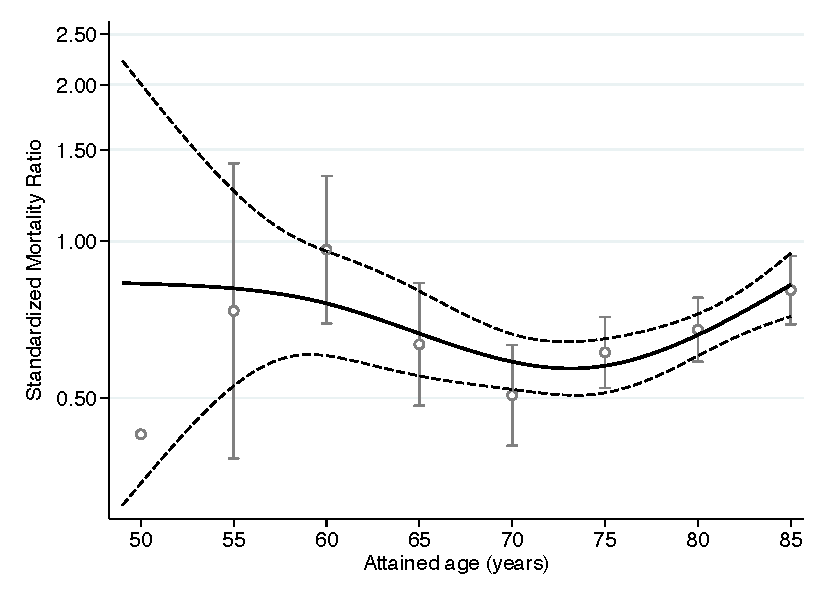
\includegraphics[width=\linewidth]{figures/smr_cage.pdf}
\caption[Standardized Mortality Ratio of prostate cancer by attained age]{SMRs of prostate cancer by attained age. The solid line is the model-based predicted SMR, while dashed lines are 95\% confidence intervals. The hollow circles represent the observed SMRs by 5-year categories of attained age together with 95\% confidence intervals. The confidence interval for $\SMR_{2, \LargerCdot}$ was not displayed since extremely wide, as it was based on 1 death only. Moreover, given that no deaths were observed in the category 45--49 years of attained age, the graph starts at age 50 years (see Table \ref{table:appendix_smr_table}). The vertical axis is on the natural log scale.}
\label{fig:appendix_smr_cage}
\end{figure}

\begin{figure}[p]
\centering
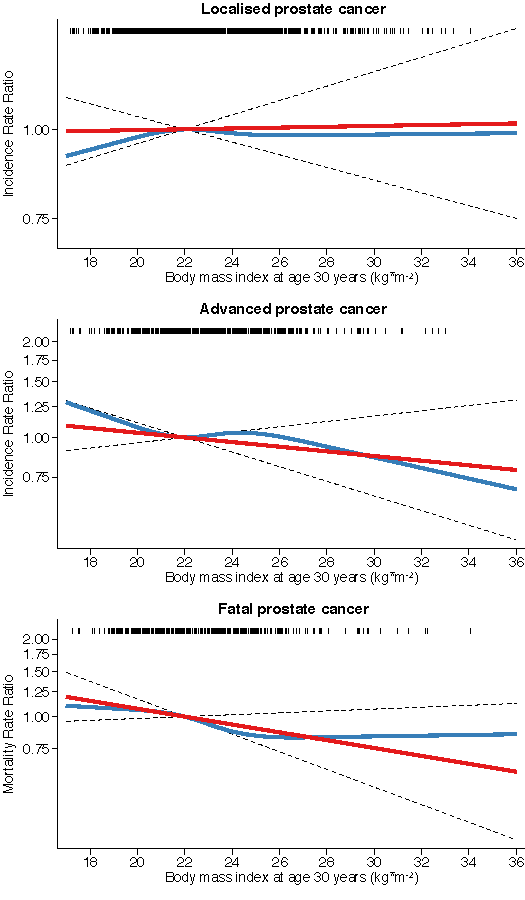
\includegraphics[width=.8\linewidth]{figures/paper1_30.pdf}
\caption[Associations of BMI at age 30 years with localized, advanced, and fatal prostate cancer]{Multivariable-adjusted associations of BMI at age 30 years (\kgmsq) with IR of localized and advanced prostate cancer, and with MR of fatal prostate cancer in the updated analysis of \citetalias{discacciati_body_2011}. BMI was modeled using RCS with 4 knots (blue line) and linearly (red line).  The referent value was set at 22 \kgmsq. Vertical lines above the curves represent cases of prostate cancer. The vertical axes are on the natural log scale.}
\label{fig:paper1_30}
\end{figure}

\begin{figure}[p]
\centering
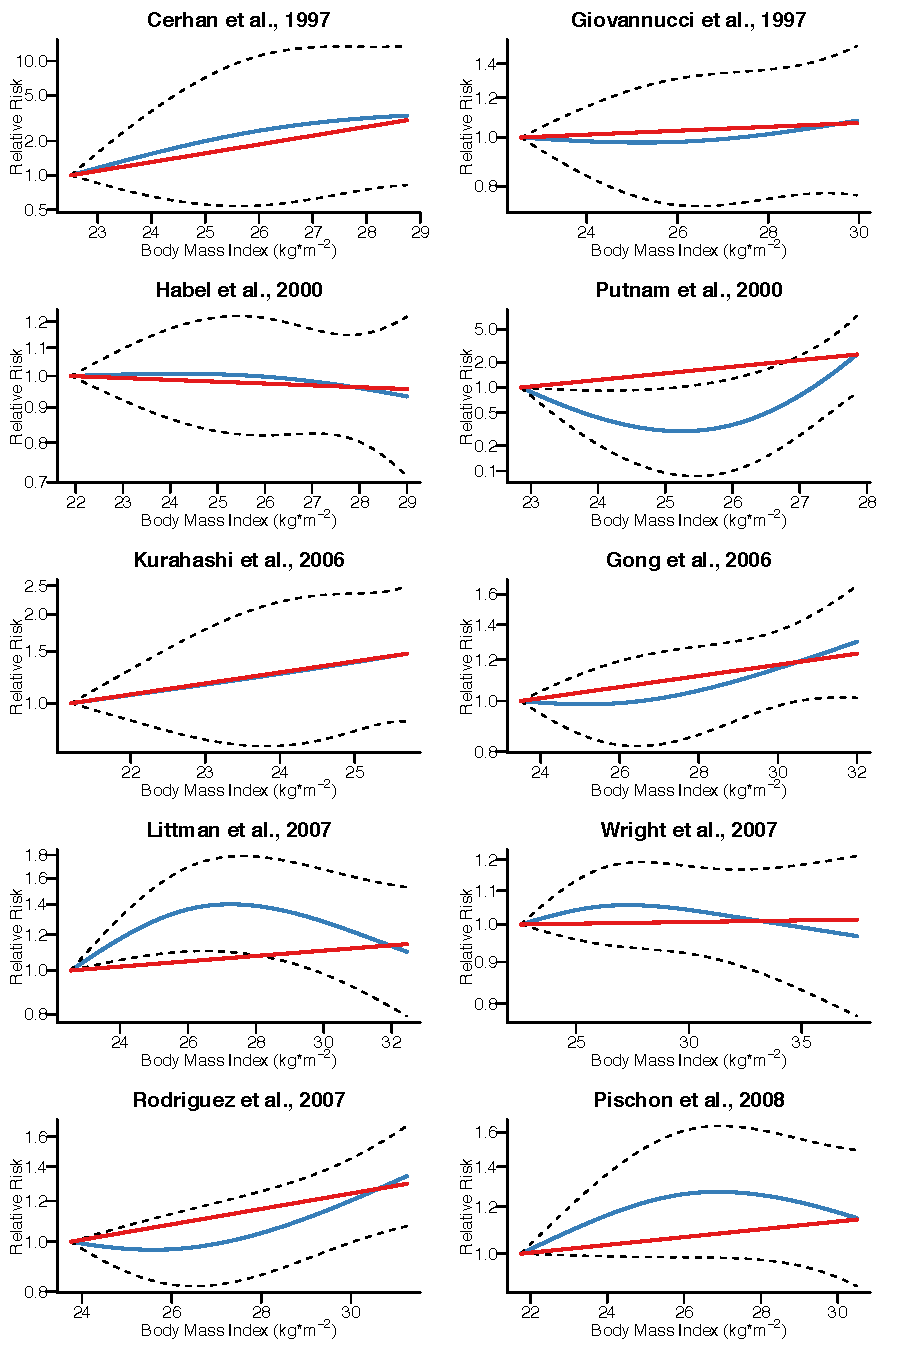
\includegraphics[width=\linewidth]{figures/ss_adv1.pdf}
\caption[Study-specific dose--response associations between BMI and incidence of advanced prostate cancer]{Study-specific dose--response associations between BMI and incidence of advanced prostate cancer in the updated meta-analysis including 18 prospective studies. BMI was modeled using RCS with 3 knots positioned at the 10th, 50th, and 90th percentiles of the overall BMI distribution (blue line) and in a linear fashion (red line). Dashed black lines represent the 95\% CI for the RCS models. The vertical axes are on the natural log scale. Figure continued on next page.}
\label{fig:ss_adv}
\end{figure}


\begin{figure}[p]
\centering
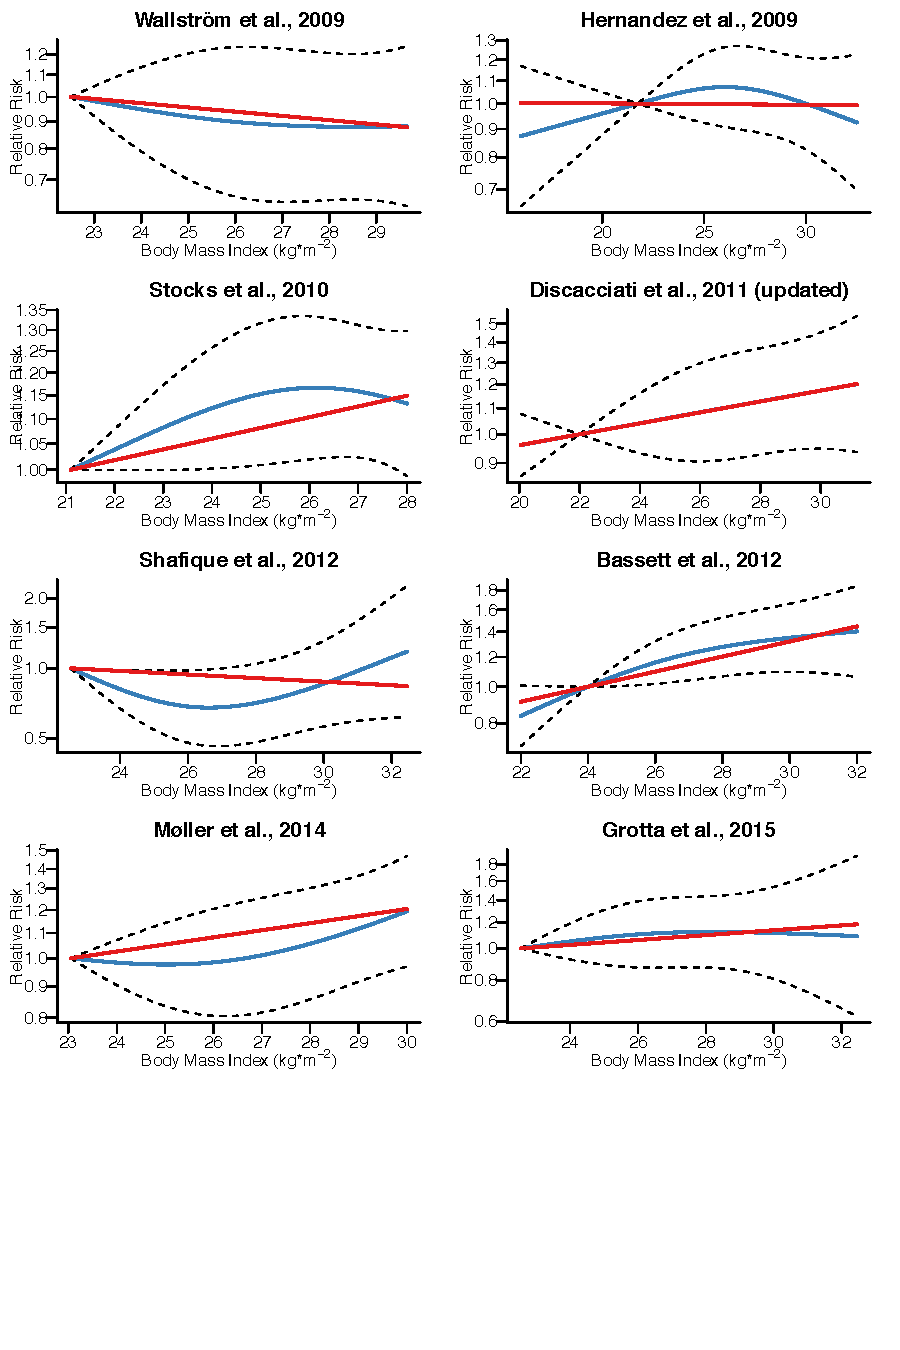
\includegraphics[width=\linewidth]{figures/ss_adv2.pdf}
\end{figure}

\begin{figure}[p]
\centering
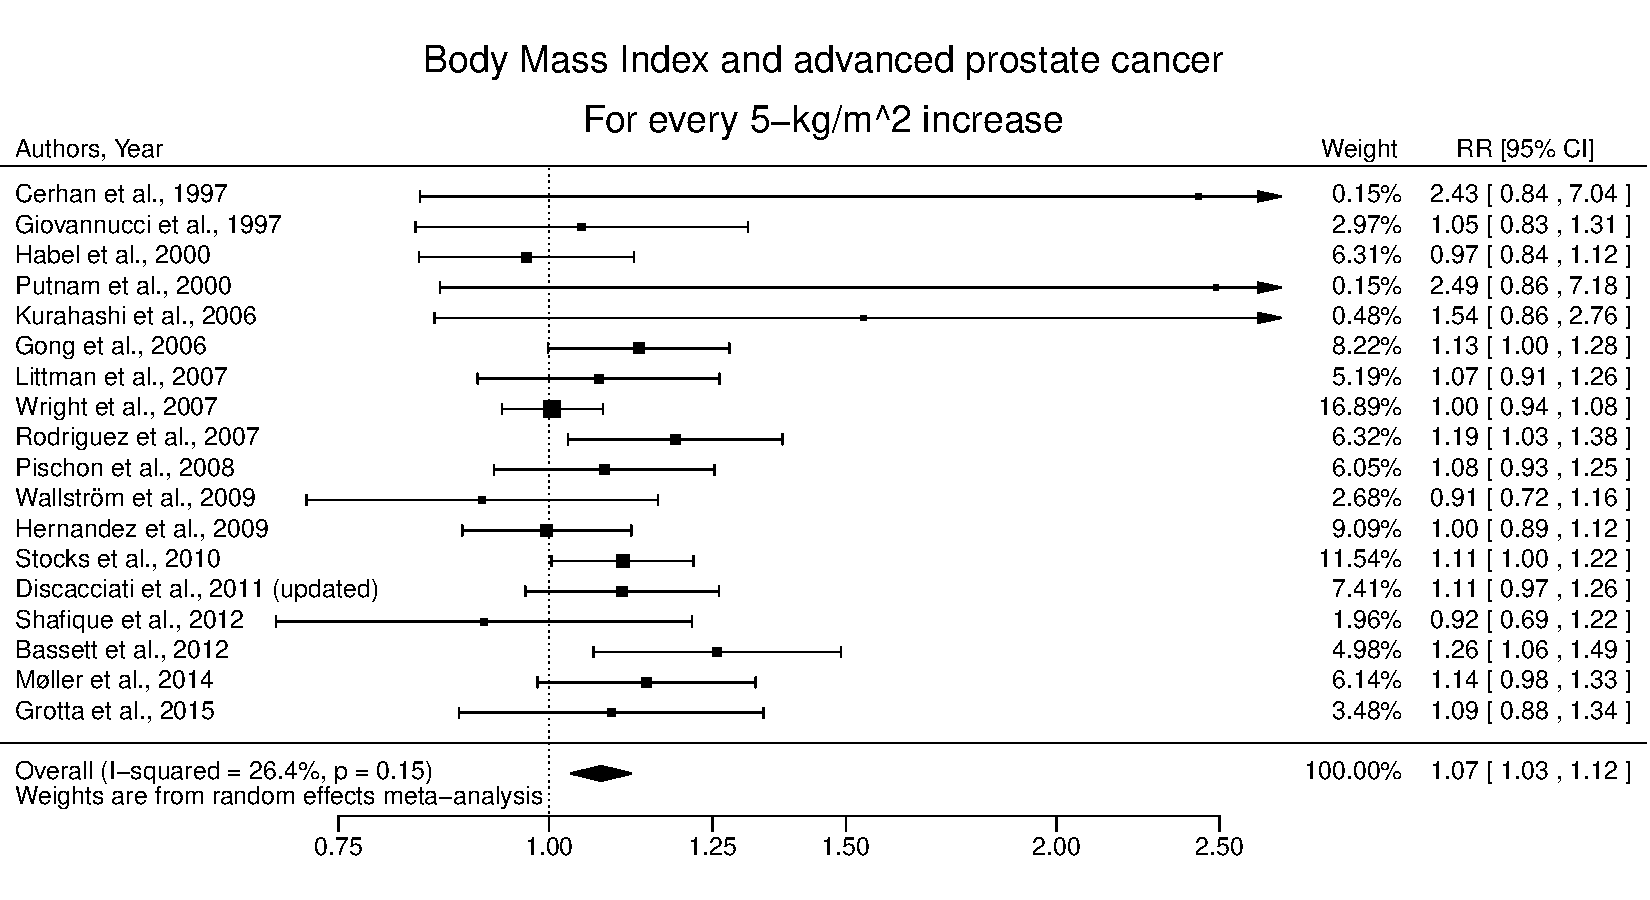
\includegraphics[width=\linewidth]{figures/fp_adv.pdf}
\caption[Forest plot for the association between BMI and incidence of advanced prostate cancer]{RRs of advanced prostate cancer for every 5-unit increment in BMI for the updated dose--response meta-analysis on 18 prospective studies. The size of each square is proportional to the weight of the study (inverse of within- plus between-study variances)}
\label{fig:fp_adv}
\end{figure}

%--tables
\chapter{Supplementary tables}

\begin{table}
\caption[Observed and expected number of prostate cancer cases in the COSM by calendar year and attained age]{Observed number of incident prostate cancer cases in the COSM by calendar year and attained age (top entry), and expected number of cases obtained by applying Swedish national rates to the COSM calendar-year and age structure (bottom entry).}
\centering
\begin{stlog}
{{\smallskip}
\HLI{10}{\TOPT}\HLI{69}
Calendar  {\VBAR}                         Attained age (years)                        
year      {\VBAR} 45-49  50-54  55-59  60-64  65-69  70-74  75-79  80-84    85+  Total
\HLI{10}{\PLUS}\HLI{69}
     1998 {\VBAR}     1      1      8     26     36     48     49      4           173
          {\VBAR}     0      3      9     19     39     46     48      4           168
          {\VBAR} 
     1999 {\VBAR}     0      5     16     28     39     61     64     10           223
          {\VBAR}     0      4     12     24     40     51     54     12           197
          {\VBAR} 
     2000 {\VBAR}     0      6     16     33     40     43     65     23           226
          {\VBAR}     0      4     14     25     41     52     54     21           212
          {\VBAR} 
     2001 {\VBAR}     0      5     16     32     59     47     61     36           256
          {\VBAR}     0      5     16     28     41     51     50     28           220
          {\VBAR} 
     2002 {\VBAR}     0      4     23     27     46     51     69     38      0    258
          {\VBAR}     0      5     17     32     40     52     50     35      0    232
          {\VBAR} 
     2003 {\VBAR}            6     26     53     63     79     72     59      5    363
          {\VBAR}            5     21     38     48     58     56     39      2    269
          {\VBAR} 
     2004 {\VBAR}            7     15     50     57     74     72     47      7    329
          {\VBAR}            5     25     47     56     63     55     37      5    293
          {\VBAR} 
     2005 {\VBAR}            4     28     47     77     60     76     51     13    356
          {\VBAR}            3     23     47     55     56     54     40      9    288
          {\VBAR} 
     2006 {\VBAR}            2     22     34     58     49     49     40     21    275
          {\VBAR}            2     23     47     51     50     48     36     13    269
          {\VBAR} 
     2007 {\VBAR}            0     21     57     57     58     36     51     29    309
          {\VBAR}            1     20     43     54     46     45     34     13    256
          {\VBAR} 
     2008 {\VBAR}                  19     52     75     39     49     35     34    303
          {\VBAR}                  16     43     51     44     43     32     16    246
          {\VBAR} 
     2009 {\VBAR}                  15     70     72     49     59     47     31    343
          {\VBAR}                  14     50     65     55     48     33     18    284
          {\VBAR} 
     2010 {\VBAR}                   9     52     57     59     54     30     20    281
          {\VBAR}                   9     43     61     52     44     32     16    257
          {\VBAR} 
     2011 {\VBAR}                   7     41     63     61     39     45     19    275
          {\VBAR}                   5     41     62     51     39     31     18    247
          {\VBAR} 
     2012 {\VBAR}                   5     28     63     48     46     32     21    243
          {\VBAR}                   2     34     58     49     34     27     18    221
          {\VBAR} 
    Total {\VBAR}     1     40    246    630    862    826    860    548    200  4,213
          {\VBAR}     1     37    227    561    761    776    722    441    128  3,656
\HLI{10}{\BOTT}\HLI{69}
\nullskip}
\end{stlog}
\label{table:appendix_sir_table}
\end{table}


\begin{table}
\caption[Observed and expected number of prostate cancer deaths in the COSM by calendar year and attained age]{Observed number of prostate cancer deaths in the COSM by calendar year and attained age (top entry), and expected number of deaths obtained by applying Swedish national rates to the COSM calendar-year and age structure (bottom entry).}
\centering
\begin{stlog}
{\HLI{10}{\TOPT}\HLI{69}
Calendar  {\VBAR}                         Attained age (years)                        
year      {\VBAR} 45-49  50-54  55-59  60-64  65-69  70-74  75-79  80-84    85+  Total
\HLI{10}{\PLUS}\HLI{69}
     1998 {\VBAR}     0      0      0      1      0      1      0      0             2
          {\VBAR}     0      0      1      2      6     12     18      2            43
          {\VBAR} 
     1999 {\VBAR}     0      0      0      0      1      1      3      0             5
          {\VBAR}     0      0      1      2      6     12     19      7            47
          {\VBAR} 
     2000 {\VBAR}     0      0      1      2      1      2      8      3            17
          {\VBAR}     0      0      1      3      6     12     20     12            53
          {\VBAR} 
     2001 {\VBAR}     0      0      0      1      4      3     14      4            26
          {\VBAR}     0      0      1      3      6     11     19     16            56
          {\VBAR} 
     2002 {\VBAR}     0      0      1      7      1      5      8     11      0     33
          {\VBAR}     0      0      1      2      4     11     17     20      0     56
          {\VBAR} 
     2003 {\VBAR}            1      1      5      1      7     15     20      2     52
          {\VBAR}            0      1      3      5     13     21     23      3     69
          {\VBAR} 
     2004 {\VBAR}            0      1      3      4      6     14     12      7     47
          {\VBAR}            0      1      2      7     11     18     23      8     70
          {\VBAR} 
     2005 {\VBAR}            0      1      2      6      9     10     16      3     47
          {\VBAR}            0      1      3      6     11     18     23     11     73
          {\VBAR} 
     2006 {\VBAR}            0      1      2      5      4     16     20      7     55
          {\VBAR}            0      1      3      5      9     17     24     17     77
          {\VBAR} 
     2007 {\VBAR}            0      1      1      6      6     11     23     16     64
          {\VBAR}            0      1      3      5      9     18     23     21     79
          {\VBAR} 
     2008 {\VBAR}                   0      4      5      5     12     13     17     56
          {\VBAR}                   1      3      5      8     16     24     26     82
          {\VBAR} 
     2009 {\VBAR}                   2      5      8      5      6     10     22     58
          {\VBAR}                   1      2      5      9     15     22     28     81
          {\VBAR} 
     2010 {\VBAR}                   0      1      1      6     14     18     30     70
          {\VBAR}                   0      2      5      8     15     22     30     82
          {\VBAR} 
     2011 {\VBAR}                   0      2      7      9     14     21     34     87
          {\VBAR}                   0      2      6      8     13     21     32     82
          {\VBAR} 
     2012 {\VBAR}                   0      0      2      8     11     21     30     72
          {\VBAR}                   0      2      5      8     12     22     34     84
          {\VBAR} 
    Total {\VBAR}     0      1      9     36     52     77    156    192    168    691
          {\VBAR}     0      2     12     37     82    152    255    284    209  1,034
\HLI{10}{\BOTT}\HLI{69}
\nullskip}
\end{stlog}
\label{table:appendix_smr_table}
\end{table}

\begin{sidewaystable}[]
\centering
\caption[Associations between categories of BMI at baseline age and localized, advanced, and fatal prostate cancer]{Multivariable-adjusted IRRs of localized and advanced prostate cancer, and MRRs of fatal prostate cancer by categories of BMI at baseline age in the updated analysis of \citetalias{discacciati_body_2011}.}
\label{table:paper1_1997}
\begin{adjustbox}{max width=\textwidth}
\begin{tabular}{lccccccc}
\hline
\multicolumn{8}{c}{{\bf BMI at baseline age, \kgmsq{}}}                                                                                                                                                                                                       \\ \hline
                                & {\bf \textless 21.0}         & {\bf 21.0--22.9}     & {\bf 23.0--24.9}     & {\bf 25.0--27.4}     & {\bf 27.5--29.9}     & {\bf $\ge$ 30.0}       & {\bf \begin{tabular}[c]{@{}c@{}}For every \\ 5-unit BMI\\ increment\end{tabular}} \\ \hline
{\bf Localized prostate cancer} & \multicolumn{1}{l}{} & \multicolumn{1}{l}{} & \multicolumn{1}{l}{} & \multicolumn{1}{l}{} & \multicolumn{1}{l}{} & \multicolumn{1}{l}{} & \multicolumn{1}{l}{}                                                              \\
No. of cases/person-years       & 84/21,290            & 323/61,897           & 532/115,888          & 651/136,921          & 283/68,009           & 164/42,705           & \multicolumn{1}{l}{}                                                              \\
IRR (95\% CI)                   & 0.77 (0.60--0.98)    & 1 (ref)              & 0.89 (0.77--1.02)    & 0.92 (0.79--1.06)    & 0.80 (0.67--0.95)    & 0.79 (0.64--0.98)    & ---                                                                               \\
                                &                      &                      &                      &                      &                      &                      &                                                                                   \\
{\bf Advanced prostate cancer}  &                      &                      &                      &                      &                      &                      &                                                                                   \\
No. of cases/person-years       & 30/21,290            & 91/61,897            & 208/115,888          & 202/136,921          & 111/68,009           & 65/42,705            &                                                                                   \\
IRR (95\% CI)                   & 0.89 (0.58--1.34)    & 1 (ref)              & 1.25 (0.98--1.61)    & 1.06 (0.82--1.37)    & 1.23 (0.91--1.65)    & 1.35 (0.95--1.92)    & 1.11 (0.96--1.27)                                                                 \\
                                &                      &                      &                      &                      &                      &                      &                                                                                   \\
{\bf Fatal prostate cancer}     &                      &                      &                      &                      &                      &                      &                                                                                   \\
No. of cases/person-years       & 25/23,153            & 77/68,197            & 136/127,667          & 137/150,490          & 75/74,306            & 45/36,362            &                                                                                   \\
MRR (95\% CI)                   & 0.85 (0.54--1.35)    & 1 (ref)              & 1.00 (0.76--1.33)    & 0.92 (0.69--1.23)    & 1.10 (0.78--1.54)    & 1.25 (0.83--1.89)    & 1.12 (0.95--1.32)                                                                 \\ \hline
\end{tabular}
\end{adjustbox}
\end{sidewaystable}

\begin{sidewaystable}[]
\centering
\caption[Associations between categories of BMI at age 30 years and localized, advanced, and fatal prostate cancer]{Multivariable-adjusted IRRs of localized and advanced prostate cancer, and MRRs of fatal prostate cancer by categories of BMI at age 30 years in the updated analysis of \citetalias{discacciati_body_2011}.}
\label{table:paper1_30}
\begin{adjustbox}{max width=\textwidth}
\begin{tabular}{lccccccc}
\hline
\multicolumn{8}{c}{{\bf BMI at age 30 years, \kgmsq{}}}                                                                                                                                                                                                      \\ \hline
                                & {\bf \textless 21.0} & {\bf 21.0--22.9}     & {\bf 23.0--24.9}     & {\bf 25.0--27.4}     & {\bf 27.5--29.9}     & {\bf $\ge$ 30.0}       & {\bf \begin{tabular}[c]{@{}c@{}}For every \\ 5-unit BMI\\ increment\end{tabular}} \\ \hline
{\bf Localized prostate cancer} & \multicolumn{1}{l}{} & \multicolumn{1}{l}{} & \multicolumn{1}{l}{} & \multicolumn{1}{l}{} & \multicolumn{1}{l}{} & \multicolumn{1}{l}{} & \multicolumn{1}{l}{}                                                              \\
No. of cases/person-years       & 391/81,774           & 714/144,676          & 631/139,388          & 220/59,843           & 61/13,895            & 20/7,133             & \multicolumn{1}{l}{}                                                              \\
IRR (95\% CI)                   & 0.94 (0.82--1.07)    & 1 (ref)              & 0.97 (0.87--1.08)    & 0.88 (0.75--1.04)    & 1.14 (0.87--1.50)    & 0.77 (0.48--1.21)    & 1.00 (0.90--1.12)                                                                 \\
                                &                      &                      &                      &                      &                      &                      &                                                                                   \\
{\bf Advanced prostate cancer}  &                      &                      &                      &                      &                      &                      &                                                                                   \\
No. of cases/person-years       & 133/81,774           & 247/144,676          & 220/139,388          & 86/59,843            & 14/13,895             & 7/7,133              &                                                                                   \\
IRR (95\% CI)                   & 0.97 (0.58--1.34)    & 1 (ref)              & 0.93 (0.77--1.12)    & 0.96 (0.74--1.24)    & 0.74 (0.43--1.29)    & 0.75 (0.35--1.61)    & 0.92 (0.77--1.10)                                                                 \\
                                &                      &                      &                      &                      &                      &                      &                                                                                   \\
{\bf Fatal prostate cancer}     &                      &                      &                      &                      &                      &                      &                                                                                   \\
No. of cases/person-years       & 103/89,861           & 172/159,460          & 153/152,789          & 50/65,330            & 11/15,145            & 6/7,691              &                                                                                   \\
MRR (95\% CI)                   & 1.08 (0.84--1.39)    & 1 (ref)              & 0.94 (0.75--1.17)    & 0.82 (0.59--1.14)    & 0.86 (0.46--1.61)    & 0.98 (0.43--2.26)    & 0.84 (0.67--1.04)                                                                 \\ \hline
\end{tabular}
\end{adjustbox}
\end{sidewaystable}